\begin{figure}[htbp]
\section*{ CHD8}
\centering
\begin{subfigure}[b]{0.95\textwidth}
\centering
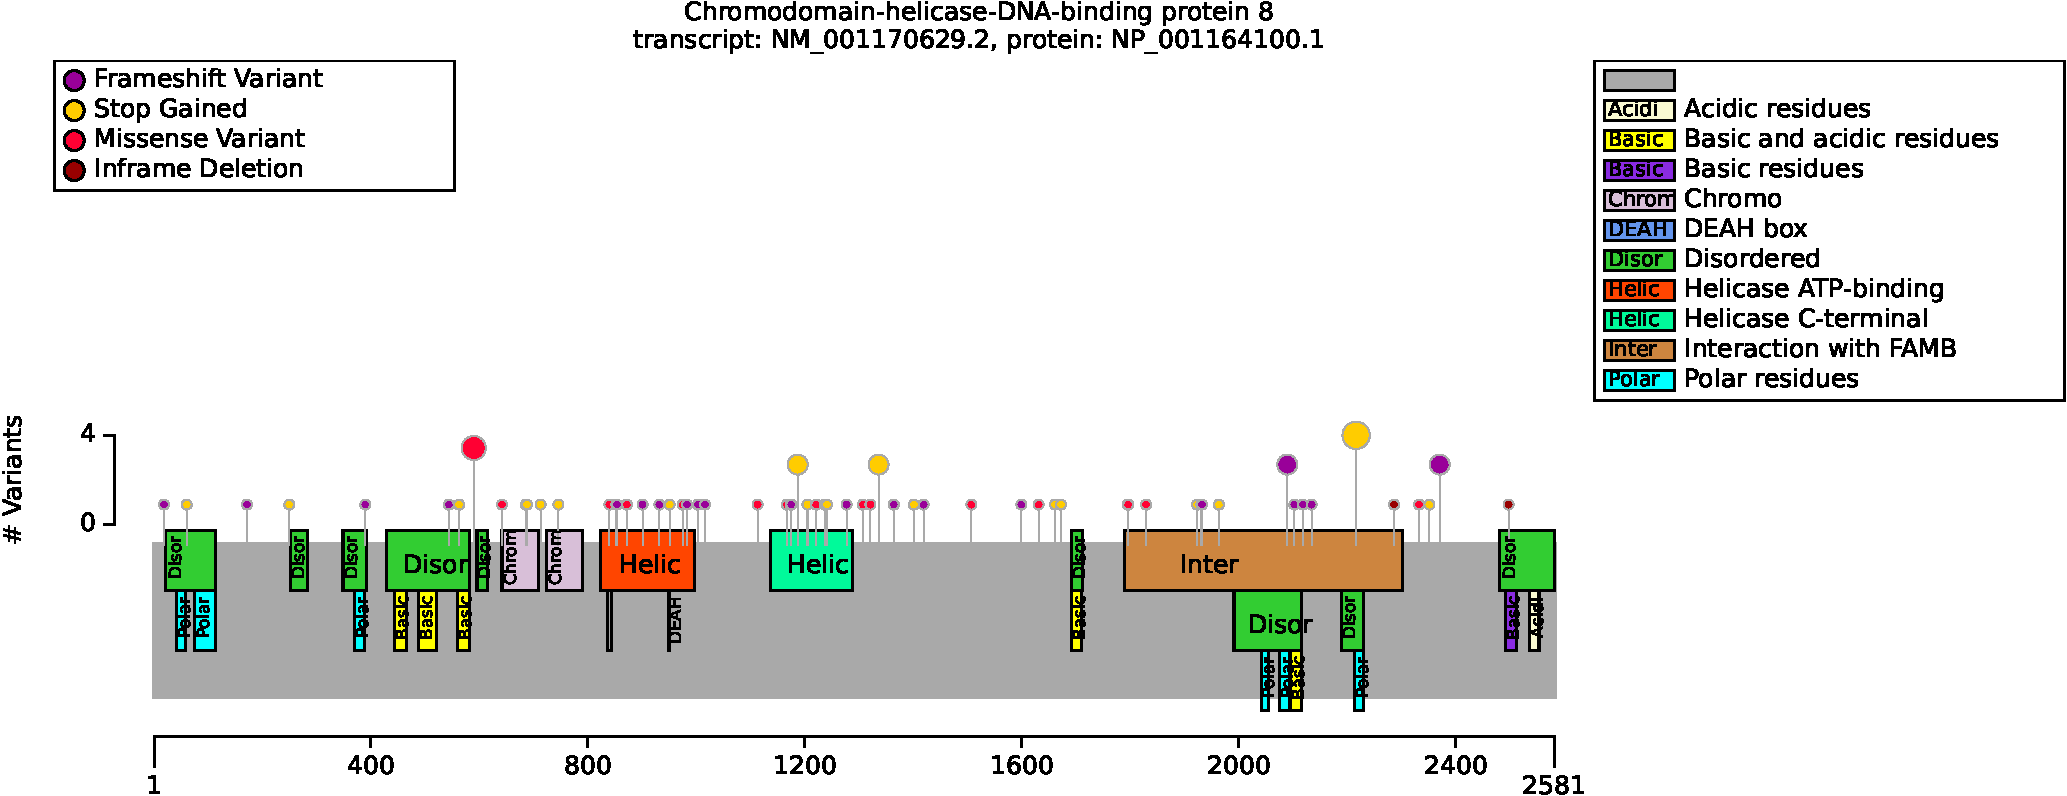
\includegraphics[width=\textwidth]{ img/CHD8_protein_diagram.pdf} 
\captionsetup{justification=raggedright,singlelinecheck=false}
\caption{Distribution of variants in CHD8}
\end{subfigure}

\vspace{2em}

\begin{subfigure}[b]{0.95\textwidth}
\centering
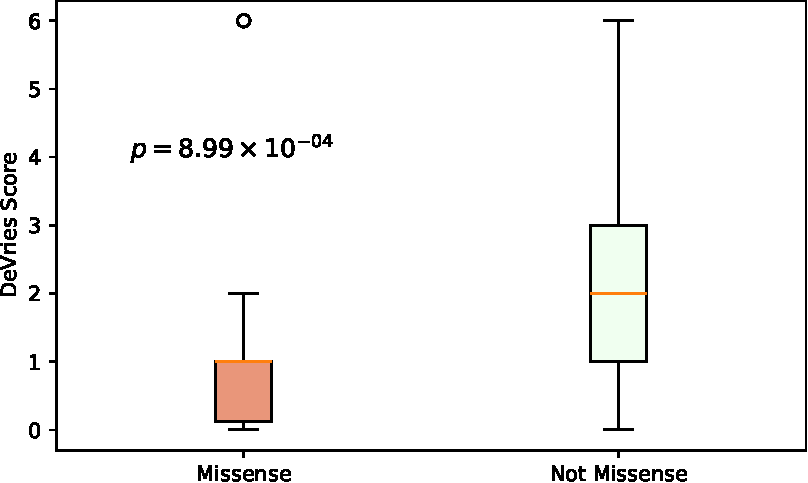
\includegraphics[width=0.3\textwidth]{img/CHD8_stats.pdf} 
\captionsetup{justification=raggedright,singlelinecheck=false}
\caption{De Vries Score to compare Missense and other variants.}
\end{subfigure}

\vspace{2em}

\begin{subfigure}[b]{0.95\textwidth}
\centering
\resizebox{\textwidth}{!}{
\begin{tabular}{llllrr}
\toprule
Genotype (A) & Genotype (B) & total tests performed & significant results\\
\midrule
Missense & Not Missense & 36 & 0\\
FEMALE & MALE & 36 & 0\\
\bottomrule
\end{tabular}
}
\captionsetup{justification=raggedright,singlelinecheck=false}
\caption{Fisher Exact Test performed to compare HPO annotation frequency with respect to genotypes.}
\end{subfigure}

\vspace{2em}

\begin{subfigure}[b]{0.95\textwidth}
\captionsetup{justification=raggedright,singlelinecheck=false}
\resizebox{\textwidth}{!}{
\begin{tabular}{llllrr}
\toprule
Description & Variable & Genotype (A) & Genotype (B) & p-value & xrefs\\
\midrule
De Vries score & De Vries score & Missense & Not Missense & $8.99\times 10^{-4}$ & \cite{PMID_36182950}\\
De Vries score & De Vries score & FEMALE & MALE & 0.006 & -\\
\bottomrule
\end{tabular}
}
\caption{De Vries Score to compare Missense and Other variants and for M/F sex differences. }
\end{subfigure}


\vspace{2em}

\caption{ The cohort comprised 79 individuals (26 females, 53 males). 1 of these individuals was reported to be deceased. 
A total of 81 HPO terms were used to annotate the cohort. Disease diagnosis: Intellectual developmental disorder with autism and macrocephaly 
(OMIM:615032).  Dingemans et al. (2022) identified a correlation between the severity of the phenotypes (as measured by a phenotype severity score termed a DeVries test) and missense variants on the CHD8 gene, 
specifically that those with a missense variant were significantly less affected than other individuals \cite{PMID_36182950}.
A total of 70 unique variant alleles were found in \textit{CHD8} (transcript: \texttt{NM\_001170629.2}, protein id: \texttt{NP\_001164100.1}).}
\end{figure}
